\vspace*{1em}

\begin{proposition}[Triangle Inequalities]\label{triangleineq}
For all $z_1,z_2 \in \cc$, the following inequalities hold.
\begin{itemize}
\item[(1)] $\abs{z_1 + z_2} \leq \abs{z_1} + \abs{z_2}$.
\item[(2)] $\abs{z_1 \pm z_2} \geq \abs{\abs{z_1} - \abs{z_2}}$. We sometimes refer to this inequality as the \cdef{reverse\ triangle\ inequality}.
\end{itemize}
\end{proposition}
\begin{proof}
\[\begin{tikzpicture}[scale=0.7]
    \draw[<->,thick] (-1,0)--(5.5,0);
	\draw[<->,thick] (0,-1)--(0,5.5);
    \fill[newblue] (5.5,5) circle (2pt) node[above]{\quad $z_1 + z_2$};
    \fill (0.5,3.5) circle (2pt) node[above]{$z_1$};
    \draw[->,>=stealth,thick] (0,0) -- (0.5,3.5);
    \draw[->,>=stealth,thick] (0,0) -- (5,1.5) node [pos=0.7, below,sloped] {$\abs{z_2}$};
	\draw[thick,dashed,newblue] (0.5,3.5)--(5.5,5);
	\draw[thick,newblue] (5,1.5)--(5.5,5) node [midway, right] {$\abs{z_1}$};
    \fill (5,1.5) circle (2pt) node[right]{$z_2$};
    \draw[->,>=stealth,thick,newblue] (0,0) -- (5.5,5) node [midway, above,sloped] {$\abs{z_1 + z_2}$};
  \end{tikzpicture}\]
\begin{itemize}
\item[(1)] A standard fact about triangles.
\item[(2)] We first assume that $\abs{z_1} \geq \abs{z_2}$. Then, $\abs{\abs{z_1} - \abs{z_2}} = \abs{z_1} - \abs{z_2}$. Now, note that
\begin{align*}
\abs{z_1} - \abs{z_2} &= \abs{z_1 \pm z_2 \mp z_2} - \abs{z_2}\\[0.5em]
 &\leq \abs{z_1 \pm z_2} + \abs{\mp z_2} - \abs{z_2},\ \text{triangle inequality}\\[0.5em]
 &= \abs{z_1 \pm z_2} + \abs{z_2} - \abs{z_2}\\[0.5em]
 &= \abs{z_1 \pm z_2}
\end{align*}
If we instead assumer $\abs{z_2} \geq \abs{z_1}$, then we do the same computation with the roles of $z_1$ and $z_2$ switched.
\end{itemize}
\vspace*{-\baselineskip}
\end{proof}

\vspace*{1em}

\begin{proposition}[Modulus is Multiplicative]\label{normmult}
For all $z,w \in \cc$ and positive integers $n$, 
\begin{itemize}
\item[(1)] $\abs{zw} = \abs{z}\abs{w}$.
\item[(2)] $\abs{z^n} = \abs{z}^n$.
\end{itemize}
\end{proposition}
\begin{proof}\hfill
\begin{itemize}
\item[(1)] Left as Problem \ref{prob 2.1a}. One proves these directly by showing that the left hand side matches the right hand side.
\item[(2)] The proof of this is by induction. $n = 1$ is a tautology, and $n = 2$ is (1) in the case $w = z$. Assume the statement is true for $n = k$, that is $\abs{z^k} = \abs{z}^k$. Then, for $n = k + 1$
\begin{align*}
|z^{k+1}| = |z^k\cdot z| &= |z^k|\abs{z},\quad \text{using (1)}\\[0.5em]
&= \abs{z}^k\abs{z},\quad \text{using the induction hypothesis}\\[0.5em]
&= \abs{z}^{k+1}
\end{align*}
Therefore we have the result by the principle of mathematical induction.
\end{itemize}
\vspace*{-\baselineskip}
\end{proof}

\vspace*{1em}

\begin{definition}[Complex Conjugation]
Given a complex number $z = x + iy$, its \cdef{(complex)\ conjugate}, denoted $\overline{z}$, is
\[\overline{z} \coloneqq x - iy\]
Geometrically, $\overline{z}$ is the reflection of $z$ about the real axis. 
\[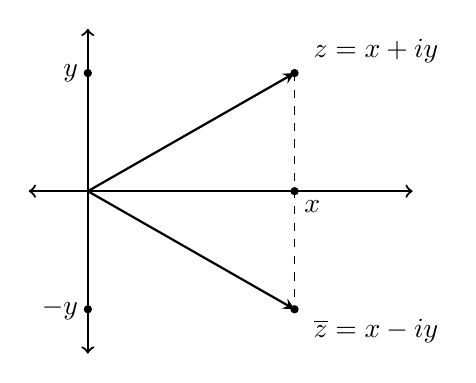
\begin{tikzpicture}[scale=0.75]
    \draw[<->,thick] (-1,0)--(5.5,0);
	\draw[<->,thick] (0,-2.75)--(0,2.75);
    \fill (3.5,2) circle (2pt) node[above right]{\ $z = x+iy$};
    \draw[->,>=stealth,thick] (0,0) -- (3.5,2);
    \fill (3.5,-2) circle (2pt) node[below right]{\ $\overline{z} = x-iy$};
    \draw[->,>=stealth,thick] (0,0) -- (3.5,-2);
    \draw[-,dashed] (3.5,2) -- (3.5,-2);
    \fill (3.5,0) circle (2pt) node[below right]{$x$};
    \fill (0,2) circle (2pt) node[left]{$y$};
    \fill (0,-2) circle (2pt) node[left]{$-y$};
  \end{tikzpicture}\]
\end{definition}

\vspace*{1em}

\begin{proposition}[Properties of Conjugation]\label{conjprop}
For all pairs $z,w \in \cc$, we have
\begin{itemize}
\item[(1)] $\overline{\overline{z}} = z$
\item[(2)] $\abs{\overline{z}} = \abs{z}$
\item[(3)] $\overline{z + w} = \overline{z} + \overline{w}$
\item[(4)] $\overline{zw} = \overline{z}\ \overline{w}$
\item[(5)] $z\overline{z} = \abs{z}^2$
\item[(6)] $\Re z = \dfrac{z + \overline{z}}{2}$ and $\Im z = \dfrac{z - \overline{z}}{2i}$
\item[(7)] $z \in \rr$ if and only if $z = \overline{z}$
\end{itemize}
\end{proposition}
\begin{proof}
(1) -- (3) is clear geometrically. (4), (6) and (7) are left as Problem \ref{prob 2.1}, (7) can be proved using (6) and can also be deduced geometrically. One proves these directly by showing that the left hand side matches the right hand side.
\begin{itemize}
\item[(5)] Let $z = x + iy$, then
\begin{align*}
z\overline{z} &= (x + iy)(x - iy)\\[0.5em]
&= x^2 - ixy + iyx - i^2y^2\\[0.5em]
&= x^2 + y^2 + i(yx - xy)\\[0.5em]
&= x^2 + y^2\\[0.5em]
&= \abs{z}^2\\[-1em]
\end{align*}
\end{itemize}
\vspace*{-\baselineskip}
\end{proof}

%\vspace*{1em}

\begin{discussion}
Proposition \ref{conjprop} (5) gives us a nice formula for $z^{-1}$ for $z\in \cc^*$. For such a $z$, we have $z\overline{z} = \abs{z}^2$, which gives us
\[z^{-1} = z^{-1}\cdot \frac{z\overline{z}}{\abs{z}^2} = \frac{\overline{z}}{\abs{z}^2}\]
This tells us that $z^{-1}$ is just a scaled $\overline{z}$, which means, geometrically speaking, $z^{-1}$ lies on the line passing through the origin and $\overline{z}$.
\end{discussion}

\vspace*{1em}

Recall that every non-zero point $(x,y) \in \rr^2$ can be re-written in polar coordinates $(r,\theta)$ as
\[x = r\cos\theta \quad \text{and} \quad y = r\sin\theta\]
This suggests the following definition.
\begin{definition}[Polar Form]
If $(r,\theta)$ are polar coordinates for a non-zero $(x,y)$, then the \cdef{polar\ form} of a non-zero complex number $z = x + iy$ is
\[z = r(\cos\theta + i\sin\theta)\]
We sometimes abbreviate $\cos\theta + i\sin\theta$ as $\cis\theta$, so $z = r\cis\theta$.\\
\\
Evidently, $(r,\theta)$ are related to $(x,y)$ by the equations
\[\abs{z} = r \quad \text{and} \quad \cos\theta = \frac{x}{r} = \frac{x}{\sqrt{x^2 + y^2}},\ \sin\theta = \frac{y}{r} = \frac{y}{\sqrt{x^2 + y^2}},\ \text{so } \tan\theta = \frac{y}{x}\]
We have to be careful and take into account which quadrant $(x,y)$ belongs to, if we think of $\theta$ with respect to its formulation using $\tan$.
\[\begin{tikzpicture}[scale=0.75]
    \draw[<->,thick] (-1,0)--(5,0);
	\draw[<->,thick] (0,-1)--(0,5);
	\fill (4,3.5) circle (2pt) node[above]{\quad $z$};
    \draw[->,>=stealth,thick] (0,0) -- (4,3.5);
    \draw[|<->|,>=stealth,thick,firebrick] (-0.2478,0.2832) -- (3.752,3.783) node [fill=white, midway, sloped] {$r$};
    \draw
    (4,3.5) coordinate (a)
    -- (0,0) coordinate (b)
    -- (0.5,0) coordinate (c)
    pic["$\color{firebrick}\theta$", ->,>=stealth,thick, draw=firebrick, angle eccentricity=1.3, angle radius=1cm]
    {angle=c--b--a};
  \end{tikzpicture}\]
Since $\sin$ and $\cos$ are periodic functions, $\theta$ is not unique (you can replace $\theta$ with $\theta + 2\pi$). Each possible value of $\theta$ is called an \cdef{argument\ of} {\color{blue}$z$}, and the set of all such $\theta$ is denoted as $\arg z$. That is,
\[\arg z = \setp{\arctan(y/x) + 2k\pi}{k \in \zz}\]
The polar form, specifically $\theta$ is unique, as soon as we specify bounds on $\theta$. The unique argument in the interval $(-\pi,\pi]$ is called the \cdef{principal\ argument} denoted $\parg z$.\\
\\
Notice that we can then write
\[\arg z = \setp{\parg z + 2k\pi}{k \in \zz}\]
\end{definition}

%\vspace*{1em}

\begin{definition}[Euler's Formula]\label{eulerform}
$e^{i\theta} \coloneqq \cis\theta = \cos\theta + i\sin\theta$. Therefore $\abs{e^{i\theta}} = 1$.
\end{definition}
\begin{proof}[Remark on Definition \ref{eulerform}]\renewcommand{\qedsymbol}{}
This is for now a stopgap, defining $e^{i\theta}$ in this way. In a few weeks, we'll see that this is truly an equality of holomorphic functions. Euler deduced this by looking at the Taylor series expansion of these functions. We haven't built or discussed enough machinery to give this reasoning a solid foundation yet. 
\end{proof}

%\vspace*{1em}

Using Euler's formula, one can write the polar form of a non-zero complex number, even more succinctly in its \cdef{exponential\ form}
\[z = re^{i\theta}\]
\begin{example}\hfill
\begin{itemize}[itemsep=1em]
\item[(1)] Exponential form of $1 + i$, 
\[\abs{1 + i} = \sqrt{1^2 + 1^2} = \sqrt{2}\quad \text{and} \quad \parg z = \arctan(1) = \frac{\pi}{4}\]
So, $1 + i = \sqrt{2}e^{i\pi/4}$.
\[\begin{tikzpicture}[scale=1.5]
    \draw[<-,thick] (-1.5,0)--(-1,0);
	\draw[->,thick] (0,1)--(0,1.5);
	\draw[->,thick] (1,0)--(1.5,0);
	\draw[<-,thick] (0,-1.5)--(0,-1);
	\fill[teal] (1,1) circle (0.8pt) node[above right]{\color{teal}$1+i$};
    \node (a) at (1,1) {};
    \node (b) at (0,0) {};
    \node (c) at (0.5,0) {};
    \draw pic["{\footnotesize$\color{teal}\theta = \dfrac{\pi}{4}$}", ->,>=stealth,thick, draw=teal, angle eccentricity=1.7, angle radius=1cm] {angle=c--b--a};
  \draw[->,>=stealth,teal,thick] (0,0) -- (1,1);
  \draw[->,>=stealth,firebrick,thick] (0,0) -- (1,0);
  \fill[firebrick] (1,0) circle (0.8pt) node[below]{\color{firebrick}$1$};
  \draw[->,>=stealth,firebrick,thick] (0,0) -- (0,1);
  \fill[firebrick] (0,1) circle (0.8pt) node[right]{\color{firebrick}$i$};
  \draw[->,>=stealth,firebrick,thick] (0,0) -- (-1,0);
  \fill[firebrick] (-1,0) circle (0.8pt) node[above]{\color{firebrick}$-1$};
  \draw[->,>=stealth,firebrick,thick] (0,0) -- (0,-1);
  \fill[firebrick] (0,-1) circle (0.8pt) node[left]{\color{firebrick}$-i$};
    \end{tikzpicture}\]
\item[(2)] Note that
\[1 = e^{i0} = e^{i2n\pi}\ \text{for any $n \in \zz$},\qquad i = e^{i\pi/2},\qquad -1 = e^{i\pi} = e^{i(2n+1)\pi}\ \text{for any $n \in \zz$}\]
One could write $-i = e^{i3\pi/2}$ but $3\pi/2 \neq \parg(-i)$; instead we should write $-i = e^{-i\pi/2}$.

\item[(3)] The circle $C_R(z_0)$ has a nice parametrisation 
\[C_R(z_0) = \{z = z_0 + Re^{i\theta}\ :\ 0 \leq \theta < 2\pi\}\]\\[-1.5em]
\[\begin{tikzpicture}[scale=0.75]
    \draw[<->,thick] (-1,0)--(5,0);
	\draw[<->,thick] (0,-1)--(0,5);
	\draw[->,>=stealth,thick] (0,0) -- (3,3);
    \draw[thick,indigo](3,3) circle (2);
    \draw[thick](3,3)--(5,3) node[midway, below]{$R$};
    \fill (3,3) circle (2pt);
    \node[left] at (3,3) {$z_0$};
    \draw[thick](3,3)--(2,4.732);
    \fill[indigo] (2,4.732) circle (2pt) node[above left]{$z$};
    \node (a) at (2,4.732) {};
    \node (b) at (3,3) {};
    \node (c) at (5,3) {};
    \draw pic["{\footnotesize$\theta$}", ->,>=stealth,thick,draw, angle eccentricity=1.5, angle radius=0.5cm] {angle=c--b--a};
    \node[] at (5,1) {\color{indigo}$C_R(z_0)$};
  \end{tikzpicture}\]
\end{itemize}
\vspace*{-\baselineskip}
\end{example}

%\vspace*{1em}

\begin{proposition}[Properties of Exponential Form]\label{propeuler}
Let $z = re^{i\theta}$ and $w = se^{i\phi}$ be non-zero complex numbers. Then
\begin{itemize}
\item[(1)] $zw = rs\  e^{i(\theta + \phi)}$
\item[(2)] $z^{-1} = (1/r) e^{-i\theta}$
\item[(3)] $z^n = r^n e^{in\theta}$, for any $n \in \zz$
\item[(4)] $\overline{z} = re^{-i\theta}$
\item[(5)] $z/w = (r/s)e^{i(\theta - \phi)}$
\end{itemize}
\end{proposition}
\begin{proof}\hfill
\begin{itemize}
\item[(1)] Note that
\begin{align*}
zw = (re^{i\theta})(se^{i\phi})&= rs(\cos\theta + i\sin\theta)(\cos\phi + i\sin\phi)\\[0.5em]
&= rs((\cos\theta\cos\phi - \sin\theta\sin\phi) + i(\cos\theta\sin\phi + \sin\theta\cos\phi))\\[0.5em]
&= rs(\cos(\theta + \phi) + i\sin(\theta + \phi))\\[0.5em]
&= rs\  e^{i(\theta + \phi)}
\end{align*}
\item[(2)] It suffices to show that $(re^{i\theta})((1/r) e^{-i\theta}) = 1$, for which we use (1).
\item[(3)] We first prove this result for $n \geq 0$, the result is clear for $n = 0$ and $n = 1$. Assume the result is true for $n = k$, that is $z^k = r^k e^{ik\theta}$. Then, for $n = k+1$
\begin{align*}
z^{k+1} &= z^kz\\[0.5em]
&= (r^k e^{ik\theta})(re^{i\theta})\ \text{using the induction hypothesis}\\[0.5em]
&= r^{k+1} e^{ik\theta+\theta}\ \text{by (1)}\\[0.5em]
&= r^{k+1} e^{i(k+1)\theta}
\end{align*}
Therefore we have the result by the principle of mathematical induction.\\[0.5em]
Suppose $n<0$ instead, then write $n = -m$ for a positive $m>0$. Now, we can apply the first case to $z^n \coloneqq (z^{-1})^m$ to get our result.
\item[(4)] Using $z\overline{z} = \abs{z}^2 = r^2$, we get that $\overline{z} = r^2z^{-1}$, and the result follows from (2).
\item[(5)] Recall $z/w = zw^{-1}$, and the result follows from (2) and (1).
\end{itemize}
\vspace*{-\baselineskip}
\end{proof}

\vspace*{1em}

\begin{example}
Let's use this to compute $(1+i)^{2021}$, then
\begin{align*}
(1 + i)^{2021} &= (\sqrt{2} e^{i\pi/4})^{2021}\\[0.5em]
&= (\sqrt{2} e^{i\pi/4})^{2020}(\sqrt{2} e^{i\pi/4})\\[0.5em]
&= (\sqrt{2})^{2020} (e^{i2020\pi/4})(1 + i)\\[0.5em]
&= 2^{1010} (e^{i505\pi})(1 + i)\\[0.5em]
&= -2^{1010}(1 + i)
\end{align*}
\end{example}

%\vspace*{1em}

\begin{example}[in-class]
Compute $(1+i\sqrt{3})^{101}$.
\end{example}
\begin{proof}[Answer]
We first note that $|1 + i\sqrt{3}| = \sqrt{1^2 + (\sqrt{3})^2} = \sqrt{4} = 2$, and since $1 + i\sqrt{3}$ lies in the first quadrant of the complex plane
\[\parg z = \arctan(\sqrt{3}) = \frac{\pi}{3}\]
Therefore
\[1+i\sqrt{3} = 2e^{i\pi/3}\]
and so
\begin{align*}
(1+i\sqrt{3})^{101} &= (2e^{i\pi/3})^{101}\\[0.5em]
 &= (2e^{i\pi/3})^{99}(2e^{i\pi/3})^{2}\\[0.5em]
 &= 2^{99}e^{i33\pi}(1+i\sqrt{3})^{2}\\[0.5em]
 &= -2^{99}(1-3 +2i\sqrt{3}),\quad \text{since $33$ is odd}\\[0.5em]
 &= -2^{99}(-2 +2i\sqrt{3})\\[0.5em]
 &= 2^{100}(1- i\sqrt{3})
\end{align*}
\end{proof}

\vspace*{1em}

\begin{discussion}
Proposition \ref{propeuler} (1) gives us a nice geometric interpretation of complex multiplication. If $z = re^{i\theta}$ and $w = se^{i\phi}$, then $zw = rs\  e^{i(\theta + \phi)}$. This can be interpreted as saying that $zw$ is obtained from $w$ by scaling $w$ by $\abs{z} = r$ and rotating $w$ by an angle of $\parg z$ (or vice versa).
\[\begin{tikzpicture}
    \draw[<->,thick] (-5,0)--(5,0);
	\draw[<->,thick] (0,-1)--(0,5);
	\fill[firebrick] (2.5,1.5) circle (2pt) node[above right]{$z$};
    \draw[->,>=stealth,thick,firebrick] (0,0) -- (2.5,1.5);
    \node (a) at (2.5,1.5) {};
    \node (b) at (0,0) {};
    \node (c) at (0.2,0) {};
    \draw pic["$\color{firebrick}\theta$", ->,>=stealth,thick, draw=firebrick, angle eccentricity=1.3, angle radius=1cm] {angle=c--b--a};
    
	\fill[indigo] (0.75,3) circle (2pt) node[above]{$w$};
    \draw[->,>=stealth,thick,indigo] (0,0) -- (0.75,3);
    \node (a) at (0.75,3) {};
    \node (b) at (0,0) {};
    \node (c) at (0.2,0) {};
    \draw pic["$\color{indigo}\phi$",left, ->,>=stealth,thick, draw=indigo, angle eccentricity=2, angle radius=0.5cm] {angle=c--b--a};

	\fill[forest] (-1.5,4) circle (2pt) node[above]{$zw$};
    \draw[->,>=stealth,thick,forest] (0,0) -- (-1.5,4);
    \node (a) at (-1.5,4) {};
    \node (b) at (0,0) {};
    \node (c) at (0.2,0) {};
    \draw pic["\quad$\color{forest}\theta + \phi$", ->,>=stealth,thick, draw=forest, angle eccentricity=1.2, angle radius=1.6cm] {angle=c--b--a};
%    \draw[|<->|,>=stealth,thick] (-2.158,3.754) -- (-0.6575,-0.247) node [fill=white, midway, sloped] {$\abs{z}\abs{w}$};
    \draw [decorate,decoration={brace,amplitude=10pt,mirror,raise=4pt},yshift=0pt,thick,forest]
(-1.5,4) -- (0,0) node [black,midway,left,xshift=-0.4cm,yshift=-0.2cm] {$\color{forest}rs\ $};
  \end{tikzpicture}\]
A few more interesting consequences
\begin{itemize}
\item[(1)] The \emph{unit circle} \[S^1 = \setp{z\in \cc}{\abs{z} = 1} = \{e^{i\theta}\ :\ \theta \in \rr\}\] is closed under multiplication. It's in fact an abelian group, usually denoted $U(1)$.
\item[(2)] \emph{De Moivre's Theorem}. From Proposition \ref{propeuler} (4) applied to $z = e^{i\theta}$ we get
\[(\cos\theta + i\sin\theta)^n = (\cos n\theta + i\sin n\theta)\]
\end{itemize}
\vspace*{-\baselineskip}
\end{discussion}

\vspace*{2em}

\subsection{Problems}
\vspace{0.1in}

\begin{problem}\label{prob 2.1a}
Prove Proposition \ref{normmult} (1).
\end{problem}

\vspace*{0.1in}

\begin{problem}\label{prob 2.1}
Prove the properties, other than (5), listed in Proposition \ref{conjprop}.
\end{problem}

\vspace{0.1in}

\begin{problem}\label{prob 2.2}
Prove that $z$ is either real or pure imaginary if and only if $z^2 = \overline{z}^2$.
\end{problem}

\vspace{0.1in}

\begin{problem}\label{prob 2.3}
Prove that $\abs{z} = 1$ if and only if $\overline{z} = \dfrac{1}{z}$. 
\end{problem}

\vspace{0.1in}

\begin{problem}\label{prob 2.4}
Follow the steps below to give an algebraic derivation of the triangle inequality (Proposition \ref{triangleineq} (a))
\begin{itemize}
\item[(a)] Show that
\[\abs{z_1 + z_2}^2 = (z_1 + z_2)(\overline{z}_1 + \overline{z}_2) = z_1\overline{z}_1 + (z_1\overline{z}_2 + \overline{z_1\overline{z}_2}) + z_2\overline{z}_2.\]
\item[(b)] Argue why
\[z_1\overline{z}_2 + \overline{z_1\overline{z}_2} = 2\Re(z_1\overline{z}_2) \leq 2\abs{z_1}\abs{z_2}.\]
\item[(c)] Use (a) and (b) to obtain $\abs{z_1 + z_2}^2 \leq (\abs{z_1} + \abs{z_2})^2$. Finally note how the triangle inequality follows from this.
\end{itemize}
\end{problem}

\vspace{0.1in}

\begin{problem}\label{prob 2.4a}
Let $z,w \in \cc$. 
\begin{itemize}[itemsep=1em]
\item[(a)] Prove the formula
\[\abs{z+w}^2 = \abs{z}^2 + 2 \Re z\overline{w} + \abs{w}^2\]
\item[(b)] Use (a) to deduce the \emph{parallelogram law}
\[\abs{z+w}^2 + \abs{z-w}^2 = 2\abs{z}^2 + 2\abs{w}^2\]
Give a geometric interpretation of this formula. 
\end{itemize}
\end{problem}

\vspace{0.1in}

\begin{problem}\label{prob 2.5}
Suppose $p$ is a polynomial with \emph{real coefficients}. Prove that
\begin{multicols}{2}
\begin{itemize}
\item[(a)] $\overline{p(z)} = p(\overline{z})$.
\item[(b)] $p(z) = 0$ if and only if $p(\overline{z}) = 0$.
\end{itemize}
\end{multicols}
\end{problem}

\vspace*{0.1in}

\begin{problem}\label{prob 2.7}
Find the principal argument $\parg z$ when
\begin{multicols}{2}
\begin{itemize}
\item[(a)] $-i(3 + 3i)^{-1}$.
\item[(b)] $(1 - i\sqrt{3})^6$.
\end{itemize}
\end{multicols}
\end{problem}